%%%%%%%%%%%%%%%%%%%%%%%%%%%%%%%%%%%%%%%%%%%%%%%%%%%%%%%%%%%%%%%%%%
%%%%%%%%%%%%%%%%%%%%%%%%%%% ANNEXES	 %%%%%%%%%%%%%%%%%%%%%%%%%%%%%
%%%%%%%%%%%%%%%%%%%%%%%%%%%%%%%%%%%%%%%%%%%%%%%%%%%%%%%%%%%%%%%%%%

\appendix
\chapter{Lien vers tout le code source de la chaîne de traitement \ktb{}}
L'intégralité du code produit pour le projet \ktb{}, depuis la création des documents \tei{} jusqu'à l'application Web, sont disponibles sur la plateforme d'hébergement de code GitHub.
\begin{itemize}
	\item \href{https://github.com/katabase}{Plateforme du projet}
	\item \href{https://github.com/katabase/1_OutputData}{Première étape: normalisation des documents \tei{}}
	\item \href{https://github.com/katabase/2_CleanedData}{Deuxième étape: extraction de données et normalisation}
	\item \href{https://github.com/katabase/3_WikidataEnrichment}{Troisième étape: enrichissement de données à l'aide de \wkd{}}
	\item \href{https://github.com/katabase/4_TaggedData}{Quatrième étape: création de jeux de données \json{} pour le site web}
	\item \href{https://github.com/katabase/Application}{Application web \ktb{}}
\end{itemize}

L'intégralité du code source est disponible sous licence libre (\href{https://www.gnu.org/licenses/gpl-3.0.html}{GNU GPL v3.0}, \href{https://mit-license.org/}{MIT} ou \href{https://creativecommons.org/}{Creative Commons}). Le site web peut également être consulté en ligne à \href{https://katabase.huma-num.fr/}{cette adresse}.

\chapter{Résultat des tests de l'algorithme d'extraction d'informations de \wkd{}}
\chaptermark{Résultat des tests}

Les résultats des tests présentés dans les tables ci-dessous (\ref{appendix:testisolate}, \ref{appendix:testfinal}) ont été menés sur un jeu de 200 couples \tname{} et \ttrait{}. Ils ont été choisis de façon à être représentatifs du jeu de données complet, avec une variété d'entrées semblables (personnes nobles et non nobles, entrées qui ne sont pas consacrées à des personnes...). Ce jeu de test présente également une structure et un degré de détail semblable au jeu de données complet. Il y a notamment exactement la même proportion d'entrées présentant un \ttrait{} que dans le jeu de test et le jeu final.

Les résultats en pourcentage sont toujours exprimés en \textbf{pourcentages du nombre total d'entrées requêtées} (soit 200).
\pagebreak

\begin{table}[h]
	\centering
	\begin{tabular}{>{\centering}m{3cm}m{2cm}m{2cm}m{2cm}m{2cm}m{2cm}}
		\hline
		\textbf{Type de requête} & \textbf{Noms} & \textbf{Noms et nom de famille noble} & \textbf{Noms et titre de noblesse} & \textbf{Noms et date de naissance et de mort} & \textbf{Noms et occupation} \\
		\hline
		\hline
		Avec reconstitution des prénoms & 48\% & 45.9\% & 50\% & 52.6\% & 53.1\% \\
		\hline
		Sans reconstitution des prénoms & 42\% & 40.5\% & 50\% & 52.6\% & 53.1\% \\
		\hline	
	\end{tabular}
	\caption{Tests menés avec un jeu de 200 entrées sur des paramètres isolés}
	\label{appendix:testisolate}
\end{table}

Le tableau ci-dessus (\ref{appendix:testisolate}) présente les résultats de tests menés pour isoler l'impact de chaque paramètee dans l'obtention du bon résultat. Les mêmes requêtes ont été lancées sur un jeu de test de 200 entrées de catalogue. Toutes les requêtes contient le prénom et le nom de famille complets (\enquote{Noms} dans la table). La première requête ne contient que ce paramètre, tandis que toutes les autres requêtes sont lancées avec un paramètre en plus: titre de noblesse, nom de famille noble, dates et occupation. Le fait que ces paramètres soient utilisés ne garantit pas qu'ils soient disponibles dans le jeu de données utilisé en entrée.  Ce test permet d'isoler de mieux construire l'algorithme final de recherches en plein texte sur le moteur de recherche de \wkd{}, puisqu'il permet de voir quels sont les paramètres les plus fiables.
\vfill
\clearpage


\begin{table}[h]
	\centering
	\begin{tabular}{m{10cm}m{4cm}}
		\textbf{Bons identifiants récupérés} & 65\% \\
		\hline
		\textbf{Score F1 } & 0.674 \\
		\hline
		\textbf{Précision } & 0.677 \\
		\hline
		\textbf{Rappel } & 0.670 \\
		\hline
		\textbf{Résultats certains } & 36\% \\
		\hline
		\textbf{Faux positifs parmi les éléments certains} & 8.5\% \\
		\hline
		\textbf{Total d'entrées requêtées } & 200 \\
		\hline
		\textbf{Identifiants récupérés } & 192 \\
		\hline
		\textbf{Silence } & 8 \\
		\hline
		\textbf{Temps d'exécution avec l'option \texttt{fetch} } & 88.3 secondes \\
		\hline
		\textbf{Temps d'exécution sans l'option \texttt{fetch}} & 92.49 secondes \\
	\end{tabular}
	\caption{Tests menés avec un jeu de 200 entrées sur l'algorithme final}
	\label{appendix:testfinal}
\end{table}

Le tableau ci-dessus présente les résultats d'un test évaluant les performances de l'algorithme final. Voici une explication de ces résultats:
\begin{itemize}
	\item \textit{Bons identifiants récupérés}: la proportion, exprimée en pourcentage, du nombre d'identifiants récupérés par l'algorithme qui correspondent aux identifiants récupérés manuellement
	\item \textit{Score F1}: le \gls{score F1}, soit la moyenne pondérée de la précision et du rappel. Contrairement  à la mesure ci-dessus, le score F1 prend en compte le silence et les faux négatifs, et offre donc une interprétation plus complète de la qualité du script.
	\item \textit{Précision}: la précision est une composante du \gls{score F1} qui mesure la proportion d'identifiants pertinents obtenus parmi tous les identifiants obtenus.
	\item \textit{Rappel}: le rappel est une composante du \gls{score F1} qui mesure la proportion d'identifiants pertinents obtenus parmi l'ensemble des identifiants pertinents qui existent.
	\item \textit{Résultats certains}: pour accélérer le processus de relecture, un score de certitude a été attribué à certains identifiants obtenus grâce à l'algorithme. Ce score dépend du nombre de paramètres utilisés dans la recherche qui a permis de récupérer l'identifiant. 36\% des résultats obtenus sont considérés comme certains.
	\item \textit{Faux positifs parmi les éléments certains}: le score de certitude présenté ci-dessus admet un taux d'erreur qui est ici quantifié: 8.5\% des résultats obtenus sont erronnés alors qu'ils ont été considérés comme certains (8,5\% du jeu de données total, donc).
	\item \textit{Total d'entrées requêtées}: le volume du jeu de données de test, soit 200 entrées.
	\item \textit{Identifiants récupérés}: le nombre d'identifiants obtenus, qu'ils soient corrects ou non.
	\item \textit{Silence}: le nombre d'entrées pour lesquelles aucun identifiant n'a été obtenu.
	\item \textit{Temps d'exécution avec l'option \texttt{fetch}}: le temps pris, en secondes, pour lancer l'intégralité de l'algorithme de récupération d'identifiants \wkd{} sur les 200 entrées en stockant dans des \glspl{log} les requêtes lancées et les identifiants requêtés.
	\item \textit{Temps d'exécution sans l'option \texttt{fetch}}: le temps pris, en secondes, pour lancer l'intégralité de l'algorithme de récupération d'identifiants sur les 200 entrées sans utiliser de fichiers de log.
\end{itemize}
\clearpage

\begin{table}[h]
	\centering
	\begin{tabular}{m{5cm}m{3cm}m{3cm}m{3cm}}
		\diagbox[innerwidth=5cm]{Score}{Base de con-\\naissances} & Score F1 -- recherche des candidates & Score F1 -- Lien avec le candidat & Overall linking accuracy \\
		DBPedia & 0.899 & 0.536 & 0.834 \\
		DataBNF & 0.689 & 0.726 & 0.7 \\
		Wikidata & 0.869 & 0.611 & 0.85 \\
	\end{tabular}
	\caption{Résultats du \gls{nel} de lieux dans des textes littéraires du XIXe~s. par Soudani et al. (2018)}
	\label{appendix:soudani}
\end{table}
Scores obtenus par Aicha Soudani et al. pour le liage d'entités nommées pour des lieux dans des textes littéraires français du \scl{XIX}, présentés à la conférence \textit{HumaNS’2018}\footcite[p. 4]{soudani_adaptation_2018}. Les scores F1 ne figurent pas dans l'article original, qui ne présente que la précision et le rappel. Je les ai donc calculés moi même. La méthode de calcul de l'\textit{overall linking accuracy} (\enquote{exactitude générale du liage}) n'est pas précisée dans l'article; il est seulement indiqué que \enquote{Cette mesure essaie d'évaluer l'efficacité globale du système, et non par phase, et exprime la fiabilité de REDEN pour la tâche de résolution des entités nommées.}\footcite[p. 4]{soudani_adaptation_2018}.

La méthode utilisée dans cet article est la suivante: les auteur.ice.s s'appuient fortement sur l'apprentissage machine, en identifiant d'abord des entités dans le texte à l'aide de \texttt{SEM} avant de lier les entités à différentes bases de connaissance en utilisant \texttt{REDEN}.


\chapter{Graphiques}
\begin{figure}
	\centering
	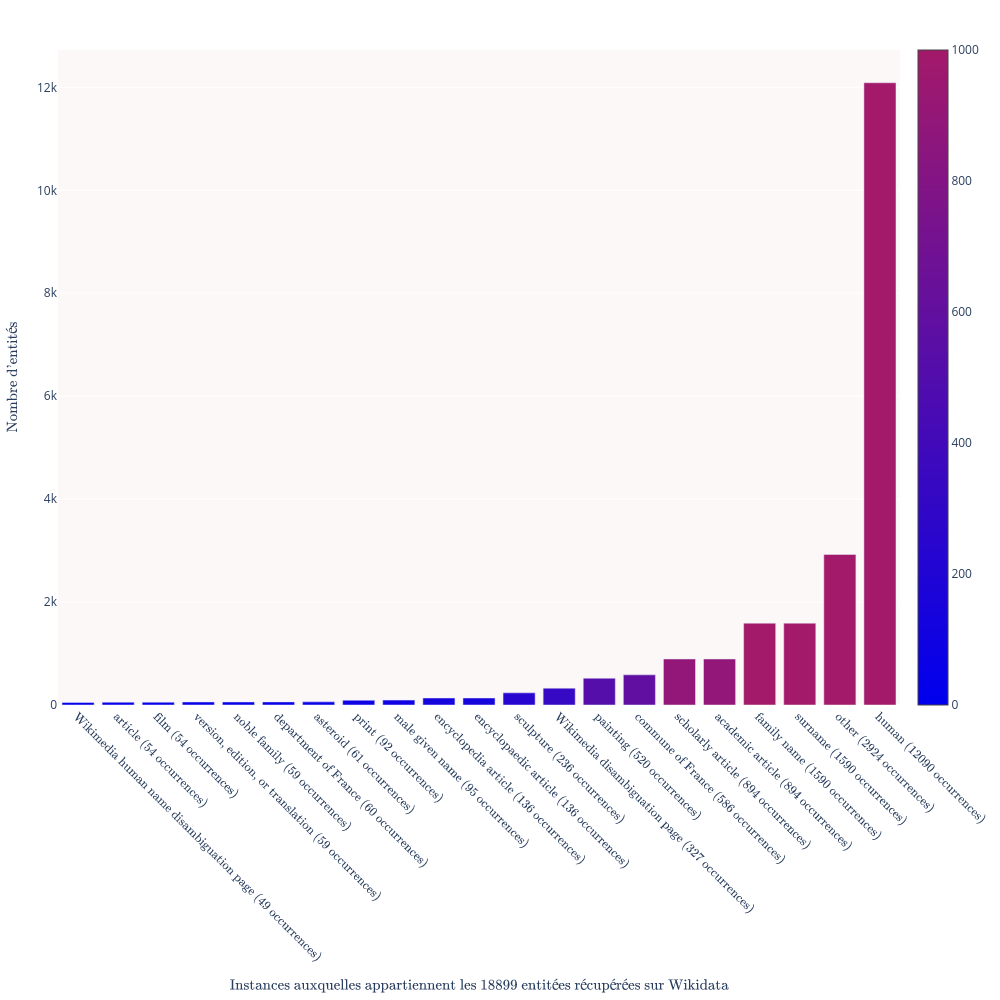
\includegraphics[width=\linewidth]{annexes/fig_wikidata_instances.png}
	\caption \\Occurrences des différentes catégories auxquelles appartiennent les entités \wkd{} liées avec les entrées de catalogues
	\label{appendix:wikidata_instances}
\end{figure}

\begin{figure}
	\centering
	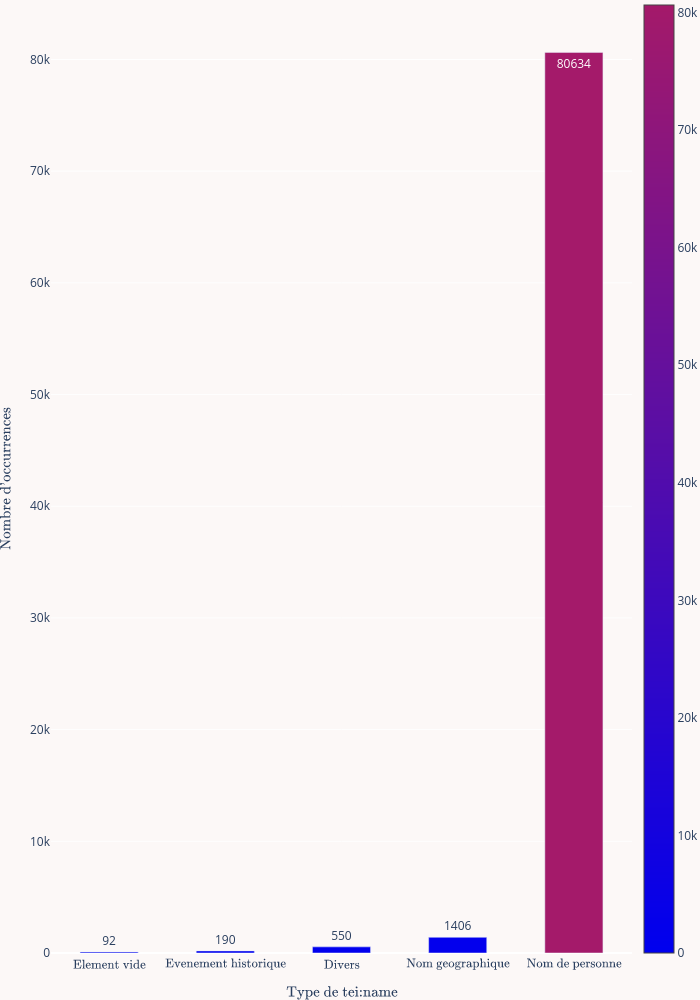
\includegraphics[width=\linewidth]{annexes/fig_teinametypes.png}
	\caption{Répartition des différents types de \tname{}}
	\label{appendix:tnametypes}
\end{figure}

\chapter{Code source et données encodées}
\begin{listing}[p]
	\begin{minted}{python}
functions = {
	"général": "general",
	"maréchal": "marshal",
	"lieutenant": "military",
	"officier": "military",
	"colonel": "military",
	"lieutenant-colonel": "military",
	"commandant": "military",
	"capitaine": "military",  # "less important" military positions
	"roi": "king",
	"empereur": "emperor",
	"president": "president",
	"homme politique": "politician",
	"président de l'assemblée": "politician",
	"orateur": "politician",
	"député": "politician",
	"secrétaire d'état": "politician",
	"sénateur": "politician",
	"écrivain": "writer",
	"auteur": "writer",
	"romancier": "writer",
	"acteur": "actor",
	"actrice": "actress",
	"cantatrice": "singer",
	"chanteur": "singer",
	"chanteuse": "singer",
	"peintre": "painter",
	"sculpteur": "sculptor",
	"statutaire": "sculptor",
	"compositeur": "composer",
	"musicien": "musician",
	"musicienne": "musician",
	"tragédien": "actor",
	"chansonnier": "chansonnier",
	"achitecte": "architect",
	"journaliste": "journalist",
	"inventeur": "inventor",
	"chimiste": "chemist",
	"connétable": "constable",
	"archevêque": "archbishop",
	"évêque": "bishop",
	"docteur": "physicist",
	"médecin": "physicist"
}		
	\end{minted}
	\caption{Table de conversion associant un métier à son équivalent normalisé}
	\label{appendix:convfunction}
\end{listing}

\clearpage
\begin{multipageminted}
	\begin{minted}{python}
dpts = [
	"ain",
	"aisne",
	"allier",
	"basses-alpes",
	"hautes-alpes",
	"alpes-maritimes",
	"annepins",
	"provence",
	"ardèche",
	"ardennes",
	"arriège",
	"arno",
	"aube",
	"aude",
	"aveyron",
	"bouches-de-l'elbe",
	"bouches-de-l'escaut",
	"bouches-de-l'yssel",
	"bpuches-de-la-meuse",
	"bouches-du-rhin",
	"bouches-du-rhône",
	"bouches-du-weser",
	"calvados",
	"cantal",
	"charente",
	"charente-inférieure",
	"cher",
	"corrèze",
	"corse",
	"côte-d'or",
	"côtes-du-nord",
	"creuse",
	"deux-nèthes",
	"deux-sèvres",
	"doire",
	"dordogne",
	"doubs",
	"drôme",
	"dyle",
	"ems-occidental",
	"ems-oriental",
	"ems-supérieur",
	"escaut",
	"eure",
	"eure-et-loir",
	"finistère",
	"forêts",
	"gard",
	"haute-garonne",
	"gers",
	"gironde",
	"hérault",
	"ille-et-villaine",
	"indre",
	"indre-et-loire",
	"isère",
	"jemappes",
	"jura",
	"landes",
	"léman",
	"loire",
	"loir-et-cher",
	"haute-loire",
	"loire-inférieure",
	"loiret",
	"lot",
	"lot-et-garonne",
	"lozère",
	"lys",
	"maine-et-loire",
	"manche",
	"marengo",
	"marne",
	"haute-marne",
	"méditerrannée",
	"mayenne",
	"meurthe",
	"meuse",
	"meuse-inférieure",
	"mont-blanc",
	"mont-tonnerre",
	"montenotte",
	"morbihan",
	"meuse",
	"moselle",
	"nièvre",
	"nord",
	"oise",
	"ombrone",
	"orne",
	"ourte",
	"paris",
	"pas-de-calais",
	"pô",
	"puy-de-dôme",
	"hautes-pyrénées",
	"basses-pyrénées",
	"pyrénées-orientales",
	"haut-rhin",
	"bas-rhin",
	"rhin-et-moselle",
	"rhône",
	"rhône-et-loire",
	"roer",
	"rome",
	"haute-saône",
	"saône-et-loire",
	"sambre-et-meuse",
	"sarre",
	"sarthe",
	"seine",
	"seine-et-marne",
	"seine-et-oise",
	"seine-inférieure",
	"sézia",
	"simplon",
	"deux-sèvres",
	"somme",
	"stura",
	"tarn",
	"tarn-et-garonne",
	"taro",
	"trasimène",
	"var",
	"vaucluse",
	"vendée",
	"vienne",
	"haute-vienne",
	"vosges",
	"yonne",
	"yssel-supérieur",
	"zuyderzée"
]		
	\end{minted}
	\caption{Liste de départements du XIXe~s. pour détecter des informations géographiques}
	\label{appendix:convdpt}
\end{multipageminted}
\clearpage

\begin{listing}[p]
	\begin{minted}{python}
countries = {
	"états-unis d'amérique": "united states of america",
	"etats-unis d'amérique": "united states of america",
	"états unis d'amérique": "united states of america",
	"etats unis d'amerique": "united states of america",
	"états-unis": "united states of america",
	"etats-unis": "united states of america",
	"etats unis": "united states of america",
	"états unis": "united states of america",
	"italie": "italy",
	"grèce": "greece",
	"canada": "canada",
	"chine": "china",
	"haïti": "haiti",
	"tobago": "tobago",
	"brésil": "brasil",
	"burkina-faso": "burkina-faso",
	"cameroun": "cameroun",
	"tchad": "tchad",
	"congo": "congo",
	"gabon": "gabon",
	"guinée": "guinea",
	"côte d'ivoire": "ivory coast",
	"mali": "mali",
	"mauritanie": "mauritania",
	"niger": "niger",
	"sénégal": "senegal",
	"madagascar": "madagascar",
	"seychelles": "seychelles",
	"tanzanie": "tanzania",
	"zanzibar": "zanzibar",
	"liban": "lebanon",
	"syrie": "syria",
	"inde": "india",
	"laos": "laos",
	"viet-nâm": "vietnam"
}	
	\end{minted}
	\caption{Table de conversion pour les pays}
	\label{appendix:convcountry}
\end{listing}

\clearpage
\begin{multipageminted}
	\begin{minted}{python}
colonies = [
	"québec",
	"ontario",
	"saint-pierre-et-miquelon",
	"mississippi",
	"missouri",
	"louisiane",
	"anguilla",
	"antigua",
	"dominique",
	"saint-domingue",
	"guadeloupe",
	"monsterrat",
	"saint-martin",
	"saint-barthélémy",
	"sainte-lucy",
	"saint-vincent-et-les-grenadines",
	"saint-eustache",
	"saint-christophe",
	"martinique"
	"guyane française",
	"guyane",
	"maroc",  # unfortunately the morocco referred to in XIXth century france is a french protectorate
	"algérie",  # same
	"algérie française",  # same
	"tunisie",  # same
	"fezzan",
	"dahomey",
	"haute-volta",
	"oubangui-chari",
	"congo français",
	"moyen-congo",
	"guinée française",
	"soudan français",
	"gorée",
	"tigi",
	"djibouti",
	"cheikh saïd",
	"comores",
	"fort-dauphin",
	"îles maurice",
	"mayotte",
	"la réunion",
	"îles éparses",
	"île amsterdam",
	"île saint-paul",
	"archipel crozet",
	"îles kerguelen",
	"castellorizo",
	"grand-liban",
	"sandjak d'alexandrette",
	"indes françaises",
	"pondichéry",
	"karikal",
	"yanaon",
	"mahé",
	"chanderngor",
	"tonkin",
	"annam",
	"cochinchine",
	"guangzhou wan",
	"shanghai",
	"guangzhou",
	"tianjin",
	"hankou",
	"clipperton",
	"nouvelle-calédonie",
	"polynésie française",
	"vanuatu",
	"nouvelles-hébrides",
	"wallis et futuna"
]
	\end{minted}
	\caption{Liste d'anciennes colonies françaises utilisées pour la détection de motifs}
	\label{appendix:convcolonie}
\end{multipageminted}
\clearpage

\begin{listing}[p]
	\begin{minted}{python}
provinces = [
	"armagnac",
	"île-de-france",
	"berry",
	"orléanais",
	"normandie",
	"languedoc",
	"lyonnais",
	"dauphiné",
	"champagne",
	"aunis",
	"saintonge",
	"poitou",
	"guyenne et gascogne",
	"bourgogne",
	"picardie",
	"anjou",
	"provence",
	"angoumois",
	"bourbonnais",
	"marche",
	"bretagne",
	"maine",
	"touraine",
	"limousin",
	"comté de foix",
	"auvergne",
	"béarn",
	"alsace",
	"artois",
	"roussillon",
	"flandre française et hainaut français",
	"franche-comté",
	"lorraine et trois-évêchés",
	"corse",
	"nivernais",
]
	\end{minted}
	\caption{Liste d'anciennes provinces françaises pour la détection de motifs}
	\label{appendix:convprov}
\end{listing}

\begin{listing}[p]
	\begin{minted}{python}
events = {
	"défense nationale": "government of national defense",
	"defense nationale": "government of national defense",
	"révolution française": "french revolution",
	"revolution francaise": "french revolution",
	"guerre de trente ans": "thirty years' war 1618 1648",
	"guerre de cent ans": "hundred years' war 1337 1453",
	"guerre de sept ans": "seven years war 1756 1763",
	"guerre": "war",
	"insurrection": "war",
	"siège de mayence": "siege of mainz",
	"siège": "siege",
	"commune": "commune",
	"défense": "battle",
	"révolution": "revolution"
}
	\end{minted}
	\caption{Table de conversion pour les évènements historiques}
	\label{appendix:convevt}
\end{listing}

\begin{listing}[p]
	\begin{minted}{python}
status = {
	"empereur": "",
	"impératrice": "",
	"géneral": "general",
	"reine": "queen",
	"roi": "king",
	"princesse": "princess",
	"prince": "prince",
	"archiduchesse": "",
	"archiduc": "",
	"duchesse": "duchess",
	"duc": "duke",
	"famille": "family",
	"seigneur": "",
	"vicomtesse": "",
	"victesse": "",
	"vicomte": "",
	"victe": "",
	"comtesse palatine": "countess palatine",
	"comtesse": "",
	"ctesse": "",
	"comte": "",
	"cte": "",
	"cardinal": "",
	"pape": "pope",
	"lord": "",
	"chevalier": "",
	"marquise": "",
	"marquis": "",
	"sire": "",
	"baronnesse": "",
	"baronne": "",
	"baron": "",
	"abbé": "",
	"madame": "",
	"mme": "",
	"monsieur": "",
	"mr": "",
	"docteur": "",
	"maréchale": "",
	"maréchal": "",
	"mademoiselle": "",
	"melle": "",
	"mlle": "",
	"sir": ""
}
	\end{minted}
	\caption{Liste de colonies pour la détection de motifs}
	\label{appendix:convstatus}
\end{listing}

\begin{listing}[p]
	\begin{minted}{python}
comp_names = {
	"arm ch": "armand-charles",
	"ch m": "charles-marie",
	"ch l f": "charles-louis-françois",
	"f m": "francois-marie",
	"fr emm.": "françois-emmanuel",
	"j ant": "jean-antoine",
	"j f": "jean-francois",
	"j m": "jean-marie",
	"j j": "jean-jacques",
	"j l": "jean-louis",
	"j b": "jean-baptiste",
	"j p": "jean-pierre",
	"j pierre": "jean-pierre",
	"l f": "louis-françois",
	"m f": "marius-felix",
	"franc rené": "francois-rené",
	"m madeleine": "marie-madeleine",
	"ph h": "philippe henri",
	"p aug": "pierre auguste",
	"p alex": "pierre alexandre",
	"p j": "pierre-jean",
	"j sylvain": "jean-sylvain",
	"l ph": "louis-philippe",
	"edm ch": "edmond-charles",
	"ch marie": "charles-marie"
}
	\end{minted}
	\caption{Table de conversion permettant de remplacer un nom abrégé composé par sa version complète}
	\label{appendix:namecomp}
\end{listing}

\begin{listing}[p]
	\begin{minted}{python}
names = {
	"ad": "adam",
	"alex": "alexandre",
	"alph": "alphonse",
	"ant": "antoine",
	"arm": "armand",
	"aug": "auguste",
	"ch": "charles",
	"cl": "claude",
	"dom": "dominique",
	"emm": "emmanuel",
	"ed": "edouard",
	"et": "etienne",
	"ét": "etienne",
	"ferd": "ferdinand",
	"fred": "frederic",
	"fr": "françois",
	"franc": "françois",
	"franç": "françois",
	"fréd": "frédéric",
	"g": "guillaume",
	"guill": "guillaume",
	"gab": "gabriel",
	"jh": "joseph",
	"jacq": "jacques",
	"jos": "joseph",
	"math": "matthieu",
	"nic": "nicolas",
	"ph": "philippe",
	"v": "victor",
	"vr": "victor",
}
	\end{minted}
	\caption{Table de conversion permettant de remplacer un nom abrégé non composé par sa version complète}
	\label{appendix:namesimp}
\end{listing}

\clearpage
\begin{multipageminted}
	\begin{minted}[breakanywhere]{python}
def rgx_abvcomp(nstr):
	"""
	try to extract an abbreviated composed first name. if there is no match, return None
	pattern
	-------
	the patterns in the example below are simplified to keep things readable
	- two strings separated by a "-" or "\s"
	- the first or second string can be a full name ([A-Z][a-z]+)
	or an abbreviation ([A-Z][a-z]*\.)
	- if the strings are separated by "\s", they must be finished by "\."
	(to be sure that we don't capture full names, i.e: "J. Ch."  can be captured,
	but not "Jean Charles")
	- complex names with 3 or more words must have "-" and at least one "\."
	- (\s|$) and (^|\s) are safeguards to avoid matching the end or beginning of another word
	examples
	--------
	matched : M.-Madeleine Pioche de la Vergne  # matched string : M.-Madeleine
	matched : C.-A. de Ferriol  # matched string : C.-A.
	matched : J. F.  # matched string : J. F.
	matched : Jean F.  # matched string : Jean F.
	matched : Jean-F.  # matched string : Jean-F.
	matched : A M  # matched string : A M
	matched : C.-Edm.-G.  # matched string : C.-Edm.-G.
	matched : Charles-Edm.-G.  # matched string : Charles-Edm.-G.
	not matched : Anne M
	not matched : Claude Henri blabla
	not matched : Claude Henri
	:param nstr: the name string used as input
	:return: the matched string if there is a match ; None if there is no match
	"""
	mo = re.search(r"(^|,|\s)[A-ZÀÂÄÈÉÊËÏÔŒÙÛÜŸ][a-zàáâäéèêëíìîïòóôöúùûüøœæç]*"
			+ "\.?-[A-ZÀÂÄÈÉÊËÏÔŒÙÛÜŸ][a-zàáâäéèêëíìîïòóôöúùûüøœæç]*\.(\s|,|$)", nstr) \
		 or re.search(r"(^|,|\s)[A-ZÀÂÄÈÉÊËÏÔŒÙÛÜŸ][a-zàáâäéèêëíìîïòóôöúùûüøœæç]*\."
			+ "-[A-ZÀÂÄÈÉÊËÏÔŒÙÛÜŸ][a-zàáâäéèêëíìîïòóôöúùûüøœæç]*\.?(\s|,|$)", nstr) \
		 or re.search(r"(^|,|\s)[A-ZÀÂÄÈÉÊËÏÔŒÙÛÜŸ]\.?\s"
			+ "[A-ZÀÂÄÈÉÊËÏÔŒÙÛÜŸ][a-zàáâäéèêëíìîïòóôöúùûüøœæç]*\.(\s|,|$)", nstr) \
		 or re.search(r"(^|,|\s)[A-ZÀÂÄÈÉÊËÏÔŒÙÛÜŸ][a-zàáâäéèêëíìîïòóôöúùûüøœæç]*\.?"
		    + "\s[A-ZÀÂÄÈÉÊËÏÔŒÙÛÜŸ]\.(\s|,|$)", nstr) \
		 or re.search(r"(^|,|\s)[A-ZÀÂÄÈÉÊËÏÔŒÙÛÜŸ]\.?\s[A-ZÀÂÄÈÉÊËÏÔŒÙÛÜŸ]\.?(\s|,|$)", nstr) \
		 or re.search(r"([A-ZÀÂÄÈÉÊËÏÔŒÙÛÜŸ]\.){2,}", nstr) \
		 or re.search(r"(^|,|\s)([A-ZÀÂÄÈÉÊËÏÔŒÙÛÜŸ][a-zàáâäéèêëíìîïòóôöúùûüøœæç]*\.?-)+"
			+ "([A-ZÀÂÄÈÉÊËÏÔŒÙÛÜŸ][a-zàáâäéèêëíìîïòóôöúùûüøœæç]*\.)(\s|,|$)", nstr) \
		 or re.search(r"(^|,|\s)([A-ZÀÂÄÈÉÊËÏÔŒÙÛÜŸ][a-zàáâäéèêëíìîïòóôöúùûüøœæç]*\.-)+"
		  	+ "([A-ZÀÂÄÈÉÊËÏÔŒÙÛÜŸ][a-zàáâäéèêëíìîïòóôöúùûüøœæç]*\.?)(\s|,|$)", nstr)
	if mo is not None:
		return mo[0]
	else:
		return None
	\end{minted}
	\caption{Fonction permettant d'identifier et d'extraire un nom abrégé composé}
	\label{appendix:rgxabvcomp}
\end{multipageminted}
\clearpage

\begin{listing}[p]
	\begin{minted}[breakanywhere]{python}
def rgx_abvsimp(nstr):
	"""
	try to extract a "simple" (not composed) abbreviated first name. if there is no match, return None
	pattern
	-------
	a capital letter (possibly followed by a certain number of lowercase letters)
	ended with a dot. (\s|$) and (^|\s) are safeguards to avoid matching the beginning
	end of another word.
	*warning* : it can also capture parts of composed abbreviated names => must be used
	in an if-elif after trying to match a composed abbreviated name
	examples
	--------
	matched : bonjour Ad.  # matched string : Ad.
	matched : J. baronne  # matched string : J.
	matched : J. F.  # matched string : J.
	matched : Jean F.  # matched string : F.
	not matched : A.-M.
	not matched : Anne M
	not matched : Hector
	:param nstr: the name string used as input
	:return:
	"""
	mo = re.search(r"(^|\s)[A-ZÀÂÄÈÉÊËÏÔŒÙÛÜŸ][a-zàáâäéèêëíìîïòóôöúùûüøœæç]*\.(\s|$|,)", nstr)
	if mo is not None:
		return mo[0]
	else:
		return None
	\end{minted}
	\caption{Fonction permettant de repérer et d'extraire un nom abrégé simple}
	\label{appendix:rgxabvsimp}
\end{listing}

\begin{listing}[p]
	\begin{minted}[breakanywhere]{python}
def rgx_complnm(nstr):
	"""
	try to extract a complete name from a string. if there is noœ match, return None
	pattern
	-------
	- an uppercase letter followed by several lowercase letters ;
	- this pattern can be repeated several times, separated by a space or "-"
	- (\s|$) and (^|\s) are safeguards to avoid matching the beginning or end of another word.
	:param nstr: the string from which a name should be extracted
	:return:
	"""
	mo = re.search(r"(^|\s)[A-ZÀÂÄÈÉÊËÏÔŒÙÛÜŸ][a-zàáâäéèêëíìîïòóôöúùûüøœæç]+"
		+ "((\s|-)[A-ZÀÂÄÈÉÊËÏÔŒÙÛÜŸ][a-zàáâäéèêëíìîïòóôöúùûüøœæç]+)*($|\s|,)", nstr)
	if mo is not None:
		return mo[0]
	else:
		return None
	\end{minted}
	\caption{Fonction permettant d'identifier et d'extraire un nom complet non abrégé}
	\label{appendix:rgxfull}
\end{listing}
\pagebreak

\clearpage
\begin{figure}[!htb]
	\begin{subfigure}{\textwidth}
		\begin{minted}{xml}
<item n="264" xml:id="CAT_000327_e264">
	<!-- ... -->
	<name type="author">Spontini (Gaspard)</name>
	<trait>
		<p>célèbre compositeur, auteur de la Vestale, né en 1779, mort en 1851.</p>
	</trait>
	<!-- ... -->
</item>
		\end{minted}
		\subcaption{La source \xmltei{}}
	\end{subfigure}
	\begin{subfigure}{\textwidth}
		\begin{minted}{python}
{
	'fname': 'gaspard ', 
	'lname': 'spontini ', 
	'nobname_sts': '', 
	'status': '', 
	'dates': '1779 1851 ', 
	'function': 'writer', 
	'rebuilt': False
}
		\end{minted}
		\caption{Le dictionnaire d'informations structurées}
	\end{subfigure}
	\begin{subfigure}{\textwidth}
		\begin{lstlisting}
gaspard spontini 1779 1851 writer
gaspard spontini 1851 writer
gaspard spontini 1779 writer
gaspard spontini writer
spontini 1779 1851 writer
spontini 1851 writer
spontini 1779 writer
spontini writer
		\end{lstlisting}
		\caption{Les recherches lancées sur l'\api{} \wkd{}}
	\end{subfigure}
	\caption{De la \tei{} à l'\api{}: document en entrée, informations extraites et chaînes de caractères recherchées}
	\label{code:apipipeline}
\end{figure}
Ci dessus (\ref{code:apipipeline}) sont présentés l'entrée et les données produites lors de l'alignement avec \wkd{}: en premier les données en entrée, ensuite les informations qui en sont extraites et enfin les différentes chaînes de caractères recherchées. Il est à noter que, dans la plupart des cas, seules une ou deux recherches sont faites sur l'\api{} avant d'obtenir un résultat; ici, huit chaînes différentes ont été construites et recherchées, ce qui représente l'intégralité de l'algorithme.
\clearpage

\begin{multipageminted}
	\inputminted[breakanywhere]{python}{./annexes/sparql_result.json}
	\caption{Exemple de réponse \sparql{} au format \json{} pour la requête \ref{code:sparql}}
	\label{appendix:sparqlout_json}
\end{multipageminted}
\clearpage

\begin{multipageminted}
	\inputminted[breakanywhere]{xml}{./annexes/sparql_result.xml}
	\caption{Exemple de réponse \sparql{} au format \xml{} pour la requête \ref{code:sparql}}
	\label{appendix:sparqlout_xml}
\end{multipageminted}
\clearpage

\begin{multipageminted}
	\begin{minted}[breakanywhere]{python}
{
	# entrées précédentes...
	"Q108438226": {
		"instance": [
			"Q3305213"
		],
		"instanceL": [
			"painting"
		],
		"gender": [],
		"genderL": [],
		"citizenship": [],
		"citizenshipL": [],
		"lang": [],
		"langL": [],
		"deathmanner": [],
		"deathmannerL": [],
		"birthplace": [],
		"birthplaceL": [],
		"deathplace": [],
		"deathplaceL": [],
		"residplace": [],
		"residplaceL": [],
		"burialplace": [],
		"burialplaceL": [],
		"educ": [],
		"educL": [],
		"religion": [],
		"religionL": [],
		"occupation": [],
		"occupationL": [],
		"award": [],
		"awardL": [],
		"position": [],
		"positionL": [],
		"member": [],
		"memberL": [],
		"nobility": [],
		"nobilityL": [],
		"workcount": [],
		"conflictcount": [],
		"img": [
			"http://commons.wikimedia.org/wiki/Special:FilePath/Louis%20de%20Frott%C3%A9.jpg"
		],
		"signature": [],
		"birth": [],
		"death": [],
		"title": [
			"Louis de Frott\u00e9 (1755-1800), g\u00e9n\u00e9ral vend\u00e9en"
		],
		"inception": [
			"1822-01-01"
		],
		"author": [],
		"authorL": [],
		"pub": [],
		"pubL": [],
		"pubplace": [],
		"pubplaceL": [],
		"pubdate": [],
		"creator": [
			"Q51077254"
		],
		"creatorL": [
			"Louise Bouteiller"
		],
		"material": [
			"Q12321255",
			"Q296955"
		],
		"materialL": [
		"canvas",
			"oil paint"
		],
		"height": [
			"216"
		],
		"genre": [
			"Q134307"
		],
		"genreL": [
			"portrait"
		],
		"movement": [],
		"movementL": [],
		"creaplace": [],
		"creaplaceL": [],
		"viafID": [],
		"bnfID": [],
		"isniID": [],
		"congressID": [],
		"idrefID": []
	},
	"Q3383960": {
		"instance": [
			"Q5"
		],
		"instanceL": [
			"human"
		],
		"gender": [
			"Q6581097"
		],
		"genderL": [
			"male"
		],
		"citizenship": [
			"Q142"
		],
		"citizenshipL": [
			"France"
		],
		"lang": [
			"Q150"
		],
		"langL": [
			"French"
		],
		"deathmanner": [],
		"deathmannerL": [],
		"birthplace": [
			"Q1148468"
		],
		"birthplaceL": [
			"Vendargues"
		],
		"deathplace": [],
		"deathplaceL": [],
		"residplace": [],
		"residplaceL": [],
		"burialplace": [],
		"burialplaceL": [],
		"educ": [],
		"educL": [],
		"religion": [],
		"religionL": [],
		"occupation": [
			"Q47064",
			"Q82955",
			"Q189290"
		],
		"occupationL": [
			"military personnel",
			"politician",
			"military officer",
			"officer"
		],
		"award": [
			"Q10855226",
			"Q11593374",
			"Q1313340"
		],
		"awardL": [
			"Grand Croix of the L\u00e9gion d'honneur",
			"Knight of the Royal and Military Order of Saint Louis",
			"names inscribed under the Arc de Triomphe",
			"Grand Cross of the Legion of Honour"
		],
		"position": [
			"Q21032625",
			"Q15904689"
		],
		"positionL": [
			"member of the Chamber of Peers",
			"Governor of Algeria"
		],
		"member": [],
		"memberL": [],
		"nobility": [
			"Q165503"
		],
		"nobilityL": [
			"baron"
		],
		"workcount": [],
		"conflictcount": [
			"1"
		],
		"img": [
			"http://commons.wikimedia.org/wiki/Special:FilePath/Berthez%C3%A8ne.JPG"
		],
		"signature": [],
		"birth": [
			"1775-03-24"
		],
		"death": [
			"1847-10-09"
		],
		"title": [],
		"inception": [],
		"author": [],
		"authorL": [],
		"pub": [],
		"pubL": [],
		"pubplace": [],
		"pubplaceL": [],
		"pubdate": [],
		"creator": [],
		"creatorL": [],
		"material": [],
		"materialL": [],
		"height": [],
		"genre": [],
		"genreL": [],
		"movement": [],
		"movementL": [],
		"creaplace": [],
		"creaplaceL": [],
		"viafID": [
			"15030322"
		],
		"bnfID": [
			"14643064j"
		],
		"isniID": [
			"0000 0000 4820 9162"
		],
		"congressID": [
			"n2005062361"
		],
		"idrefID": [
			"088623629"
		]
	},
	# entrées suivantes...
}
	\end{minted}
	\caption{Extrait de la base de connaissance constituée grâce à \sparql{} suite  à l'alignement avec des entités \wkd{}}
	\label{appendix:dbextract}
\end{multipageminted}
\clearpage

\begin{listing}[p]
	\begin{minted}{xml}
<listPrefixDef>
	<prefixDef 
		ident="wd" 
		matchPattern="(Q[0-9]+)" 
		replacementPattern="https://www.wikidata.org/wiki/$1">
		<p>
			In the <gi>body</gi>, the <att>ref</att> attributes 
			containted in <gi>name</gi> elements are pointing to to a
			<ref target="https://www.wikidata.org/wiki/">Wikidata</ref> 
			identifier by using the <code>wd:</code> prefix. This <gi>prefixDef</gi>
			allows to rebuilt the complete URL from a wikidata identifier by 
			replacing the <code>wd:</code> prefix with:
			<code>https://www.wikidata.org/wiki/</code>.
		</p>
	</prefixDef>
</listPrefixDef>
	\end{minted}
	\caption{Le \texttt{tei:listPrefixDef} décrivant le rôle du préfixe \enquote{wd} dans les catalogues}
	\label{appendix:listprefixdef}
\end{listing}

\chapter{Images}
\begin{figure}[p]
	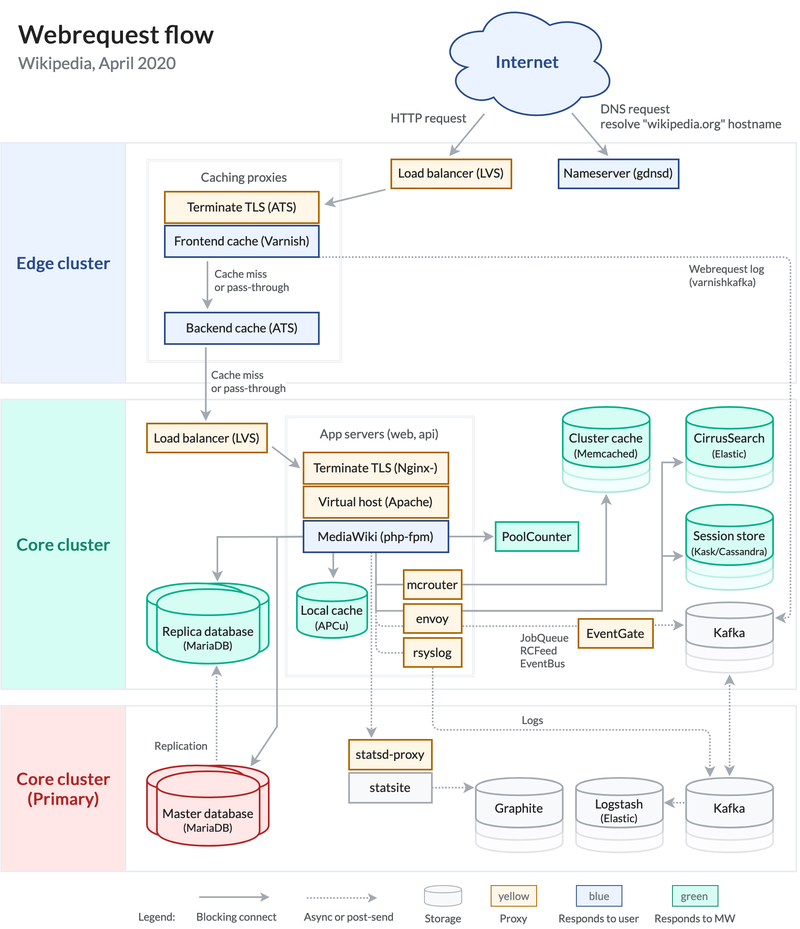
\includegraphics[width=\textwidth]{annexes/wikimedia_db_2020.png}
	\caption{L'architecture des bases de données de la \textit{Wikimedia Foundation} (schéma réalisé par Timo Tijhof en 2020, disponible dans le domaine public avec la licence Creative Commons CC0.1.0 Universal Public Domain License)}
	\label{appendix:wikimedia_db}
\end{figure}